\documentclass[../informe.tex]{subfiles}

\begin{document}
    \section{Models}
    En aquest apartat, es pot veure els valors, tant la puntuació \texttt{log(UPSM)} com el percentatge d'error de la classificació.
    
    \subsection{Models de la classe 1}
    Les 10 execucions que s'ha realitzat, ens ha donat els següents resultats:
    \begin{enumerate}
        \item \textbf{log(UPSM)}: -89814.4077531957 \ \ \ \ \ \ \ \ \textbf{Error classificació}: 50.1583 \%
        \item \textbf{log(UPSM)}: -90397.4380825399 \ \ \ \ \ \ \ \ \textbf{Error classificació}: 50.19 \%
        \item \textbf{log(UPSM)}: -90415.35102713174 \ \ \ \ \ \ \ \ \textbf{Error classificació}: 50.1583 \%
        \item \textbf{log(UPSM)}: -90389.28857008628 \ \ \ \ \ \ \ \ \textbf{Error classificació}: 50.1583 \%
        \item \textbf{log(UPSM)}: -89867.8124939057 \ \ \ \ \ \ \ \ \textbf{Error classificació}: 50.1583 \%
        \item \textbf{log(UPSM)}: -90211.85119256149 \ \ \ \ \ \ \ \ \textbf{Error classificació}: 50.1583 \%
        \item \textbf{log(UPSM)}: -90211.85119256149 \ \ \ \ \ \ \ \ \textbf{Error classificació}: 50.1583 \%
        \item \textbf{log(UPSM)}: -90450.80679248775 \ \ \ \ \ \ \ \ \textbf{Error classificació}: 50.1583 \%
        \item \textbf{log(UPSM)}: -90401.35562920943 \ \ \ \ \ \ \ \ \textbf{Error classificació}: 50.1583 \%
        \item \textbf{log(UPSM)}: -89702.37746226412 \ \ \ \ \ \ \ \ \textbf{Error classificació}: 50.1583 \%
    \end{enumerate}

    Per a poder seleccionar el millor model dels anteriors hem d'observar quin d'ells té el menor error de classificació, és a dir, el quin més encerts té.

    \medskip
    Com s'observa, casi tots els models excepte el 2 tenen el mateix error de classificació, i perquè l'error menor és el més repetit per a seleccionar el millor model s'ha d'agafar el quin tingui la puntuació \texttt{log(UPSM)} major. Per tant, el millor model és el 10è.

    \begin{figure}[H]
        \centering
        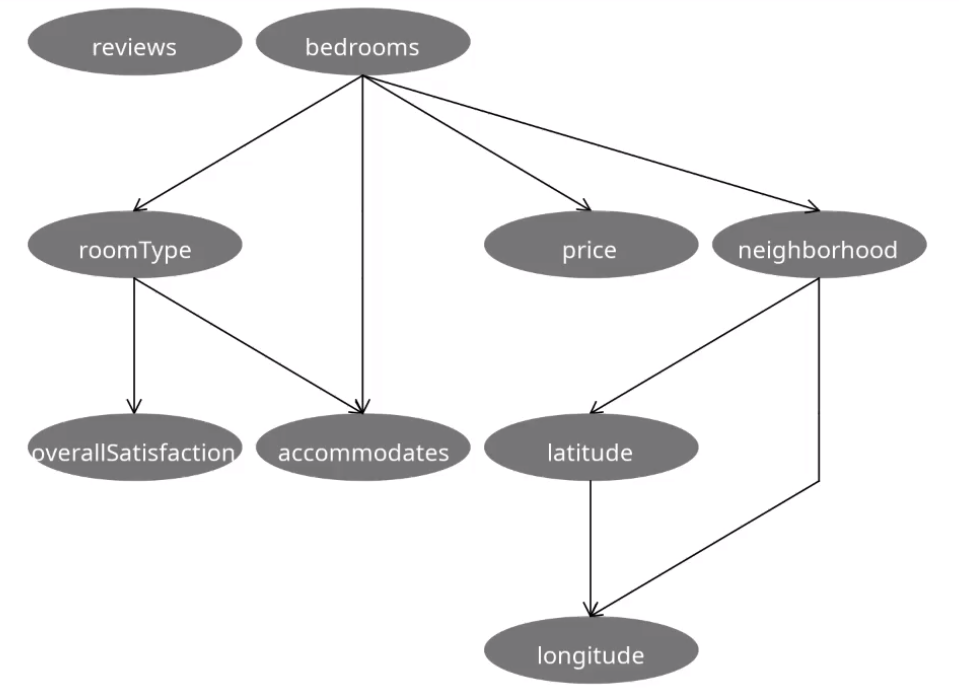
\includegraphics[width=0.7\textwidth]{model1.png}
        \caption{Millor model de la classe 1}
        \label{fig:model1}
    \end{figure}

    \medskip
    \subsection{Model de la classe 2}
    L'execució que s'ha realitzat, ja que només hi ha un model possible, és la següent:
    \begin{enumerate}
        \item \textbf{log(UPSM)}: -114260.90629096203 \ \ \ \ \ \ \ \ \textbf{Error classificació}: 50.57 \%
    \end{enumerate}

    \begin{figure}[H]
        \centering
        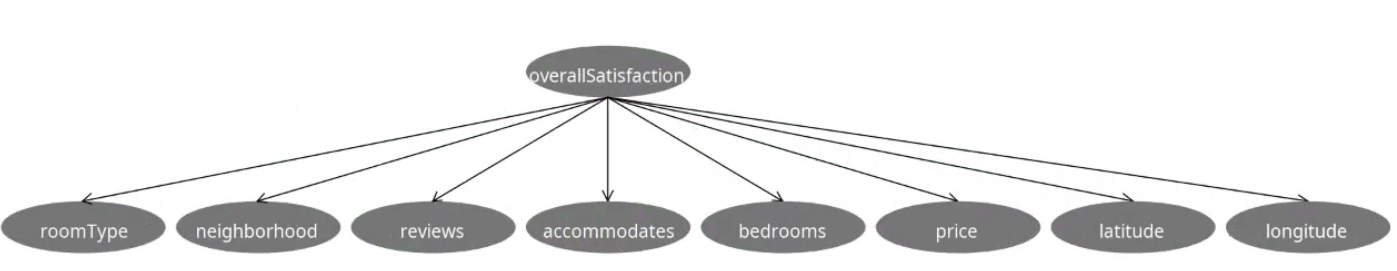
\includegraphics[width=\textwidth]{model2.png}
        \caption{Model de la classe 2}
        \label{fig:model2}
    \end{figure}

    \medskip
    \subsection{Models de la classe 3}
    Les 10 execucions que s'ha realitzat, ens ha donat els següents resultats:
    \begin{enumerate}
        \item \textbf{log(UPSM)}: -92145.77402274412 \ \ \ \ \ \ \ \ \textbf{Error classificació}: 50.2217 \%
        \item \textbf{log(UPSM)}: -93769.8023647269 \ \ \ \ \ \ \ \ \textbf{Error classificació}: 49.8417 \%
        \item \textbf{log(UPSM)}: -92947.0699716769 \ \ \ \ \ \ \ \ \textbf{Error classificació}: 49.9367 \%
        \item \textbf{log(UPSM)}: -92383.57112958582 \ \ \ \ \ \ \ \ \textbf{Error classificació}: 50.19 \%
        \item \textbf{log(UPSM)}: -93769.8023647269 \ \ \ \ \ \ \ \ \textbf{Error classificació}: 49.8417 \%
        \item \textbf{log(UPSM)}: -93355.04636895073 \ \ \ \ \ \ \ \ \textbf{Error classificació}: 50.0317 \%
        \item \textbf{log(UPSM)}: -92773.38194075429 \ \ \ \ \ \ \ \ \textbf{Error classificació}: 50 \%
        \item \textbf{log(UPSM)}: -93769.8023647269 \ \ \ \ \ \ \ \ \textbf{Error classificació}: 49.8417 \%
        \item \textbf{log(UPSM)}: -92339.30633873143 \ \ \ \ \ \ \ \ \textbf{Error classificació}: 50.0633 \%
        \item \textbf{log(UPSM)}: -92563.94627690384 \ \ \ \ \ \ \ \ \textbf{Error classificació}: 50.19 \%
    \end{enumerate}

    Per escollir el millor model de la classe 3, al igual que a la classe 1, s'ha agafat el model amb menor error de classificació.

    \medskip
    Com s'observa, tenim que els models 2, 5 i 8 tenen el mateix error de classificació i també la mateixa puntuació \texttt{log(UPSM)}, i per tant, el millor model es qualsevol d'aquests tres.

    \begin{figure}[H]
        \centering
        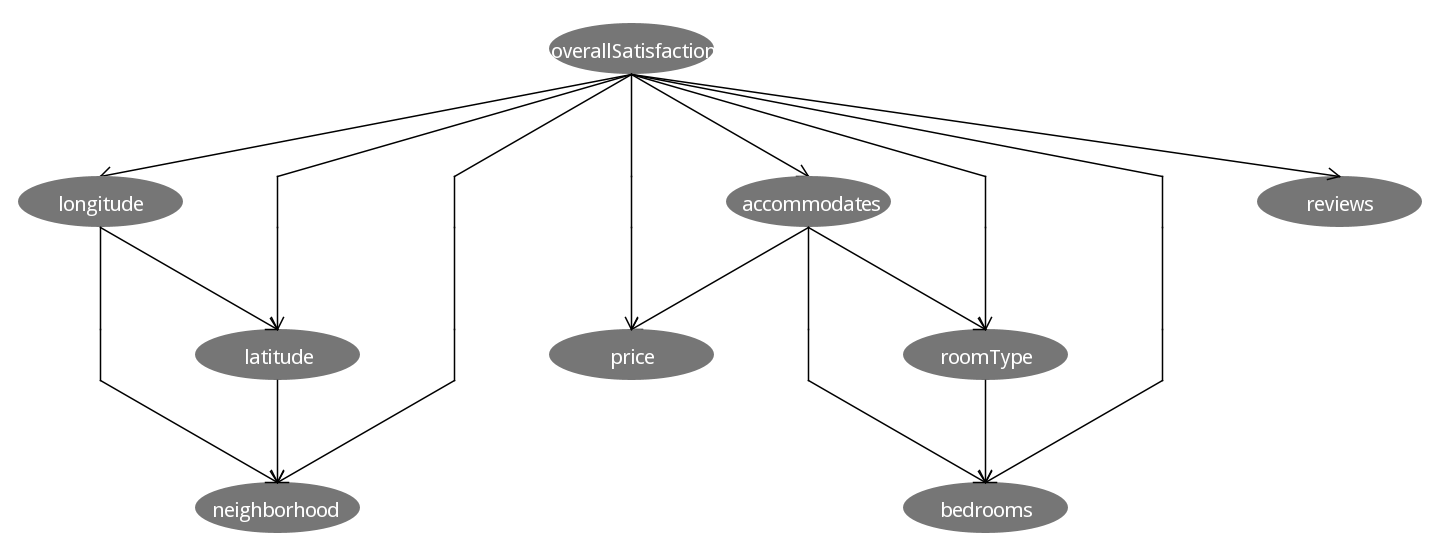
\includegraphics[width=\textwidth]{model3.png}
        \caption{Millor model de la classe 3}
        \label{fig:model3}
    \end{figure}
\end{document}